\chapter{Réalisations}
\label{Developpement}


\section{Les Projets}

\subsection{MobiSaaS}

\subsubsection{Présentation : spécifications fonctionnelles}

Le projet "MobiSaaS" s'inscrit dans la démarche d'entreprise de proposer des solutions en mode \textbf{SAAS}. Le projet consiste d'une manière générale à exposer les fonctionnalité de la solution desktop du produit "MobiAnalyst"(Fig. \ref{OffreMobiAnalyst}).

\begin{figure}[!h]
\centering
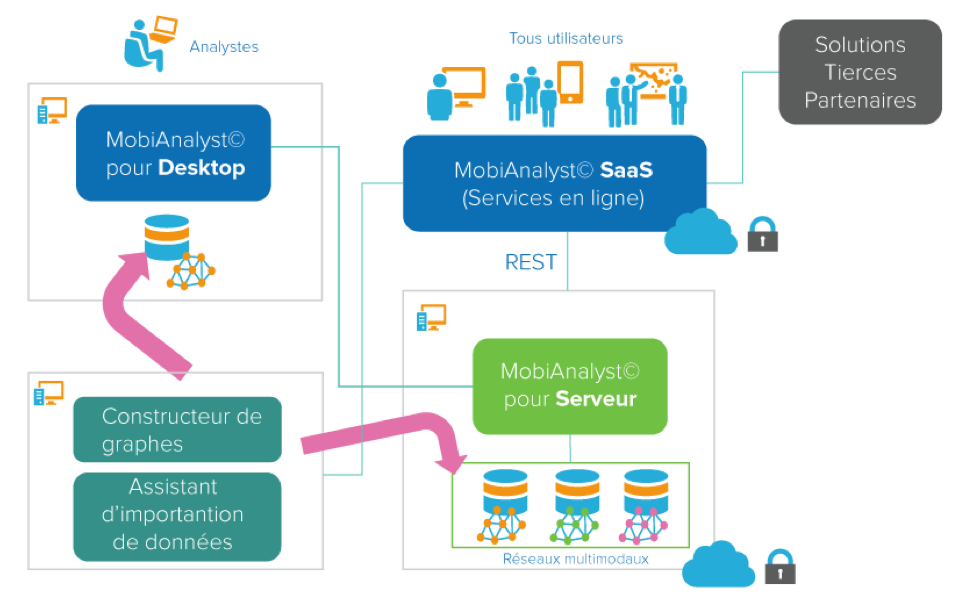
\includegraphics[width=14cm]{images/offre_MobiAnalyst.png}
\caption{\label{OffreMobiAnalyst}Offre du produit MobiAnalyst}
\end{figure} 

\subsubsection{Technologies : spécifications techniques}

\subsubsection{Objectifs / Développements}

\subsubsection{Résultats obtenus / Difficultés rencontrées}

\subsubsection{Perspectives}


\subsection{DataWizard}

\subsubsection{Présentation : spécifications fonctionnelles}

Le projet "DataWizard" ....\\

\subsubsection{Technologies : spécifications techniques}


\subsubsection{Objectifs / Développements}


\subsubsection{Résultats obtenus / Difficultés rencontrées}


\subsubsection{Perspectives}

